\documentclass[10pt,twocolumn,letterpaper]{article}
%% Welcome to Overleaf!
%% If this is your first time using LaTeX, it might be worth going through this brief presentation:
%% https://www.overleaf.com/latex/learn/free-online-introduction-to-latex-part-1

%% Researchers have been using LaTeX for decades to typeset their papers, producing beautiful, crisp documents in the process. By learning LaTeX, you are effectively following in their footsteps, and learning a highly valuable skill!

%% The \usepackage commands below can be thought of as analogous to importing libraries into Python, for instance. We've pre-formatted this for you, so you can skip right ahead to the title below.

%% Language and font encodings
\usepackage[english]{babel}
\usepackage[utf8x]{inputenc}
\usepackage[T1]{fontenc}

%% Sets page size and margins
\usepackage[a4paper,top=3cm,bottom=2cm,left=3cm,right=3cm,marginparwidth=1.75cm]{geometry}

%% Useful packages
\usepackage{amsmath}
\usepackage{graphicx}
\usepackage[colorinlistoftodos]{todonotes}
\usepackage[colorlinks=true, allcolors=blue]{hyperref}
\usepackage{natbib}
\bibliographystyle{unsrt}
%% Title
\title{
		\usefont{OT1}{bch}{b}{n}
		\normalfont \normalsize \textsc{STEM Fellowship Big Data Challenge 2020} \\ [10pt]
		\huge{The Impacts of COVID-19 on the Black Community in the United States of America} \\
		
}
\selectlanguage{english}
\usepackage{authblk}
\author[1]{Aditya Singh}
\author[1]{Flora Zhang}
\author[1]{Nishita Dahisaria}
%\author[2]{Author Four}
\affil[1]{University of British Columbia}
%\affil[2]{B University}

\begin{document}
\maketitle

\begin{abstract}
The Corona-virus is a pandemic that has quickly taken over the entire planet. It's impact has been most pronounced in USA, with the states having both the highest number of confirmed cases and deaths at the time of writing\cite{apm}. However, when examining data regarding the effect of the pandemic on different races, multiple findings reported a higher mortality rate amongst black people than any other race. This study aims to discern the reasons behind this discrepancy. 

This problem was investigated using R and MS Excel to analyse open data-sets and investigate possible relationships. Multiple regressions were performed to figure the factors that significantly affected the black population death percentage. Our findings suggest Black population\%, Population density, Median House Value, Life Expectancy, and Diabetes Prevalence to be those factors. On the other hand, Poverty was a surprising omission. 

As only data from states with above-average black populations was used, it would be interesting to see this study replicated using data from all the states of the US. 

It is unknown if the pattern acknowledged by this study is prevalent in other countries as well. Therefore, a similar study conducted on other countries with significant black minorities may also be to a worthy endeavour. 

%Ok need to add stuff about limitations and possiblities going ahead.

%Introduction/Background: Explains what problem the study examined and why. You may provide some background to the project, and the motivation behind it. Materials and Methods: Describes the data sources used and methodologies adopted for the data analysis. Key Findings/Results: Outlines the discoveries/what was observed from the analysis. When describing your results, strive to focus on the main finding(s), and list no more than two or three points. Conclusion: Provide a general interpretation of the results, specifying what is new/innovative of your project, and give any important recommendation for future research.Once you've written these, delete the keywords, edit for flow, and you have your abstract
\end{abstract} 
{\textbf{Keywords} \\
COVID-19, Coronavirus and Race, Socioeconomic and Health Factors, Black People in the USA}

\section{Introduction}

Since the first confirmed case of the corona virus on 31st December, 2019, the world has been captivated by the pandemic. Despite enjoying a brief interlude until after other countries were completely engulfed,the USA currently has the highest number of confirmed cases and deaths.  


The American government has kept records of all corona cases since late January \cite{apm}. A part of these records include the racial data of the victims of this virus. A cursory glance at this data shows that a larger than proportional number of corona patients are African-Americans, resulting in a much higher mortality rate in black people. As the biological impacts of the virus are still not fully understood, the importance of socioeconomic factors can not be understated when discussing the racial discrepancy. This prompted an investigation into what primary factors, health and otherwise, influenced this higher mortality rate the most.

In this paper, open pandemic databases were used in conjunction with demographic data provided by the state census. This data was then refined and analysed using MS Excel and R. 

Considering the current tensions in the USA, this study could also potentially be an indicator of the systemic racism prevalent in American society. 


\begin{figure}
  \centering
  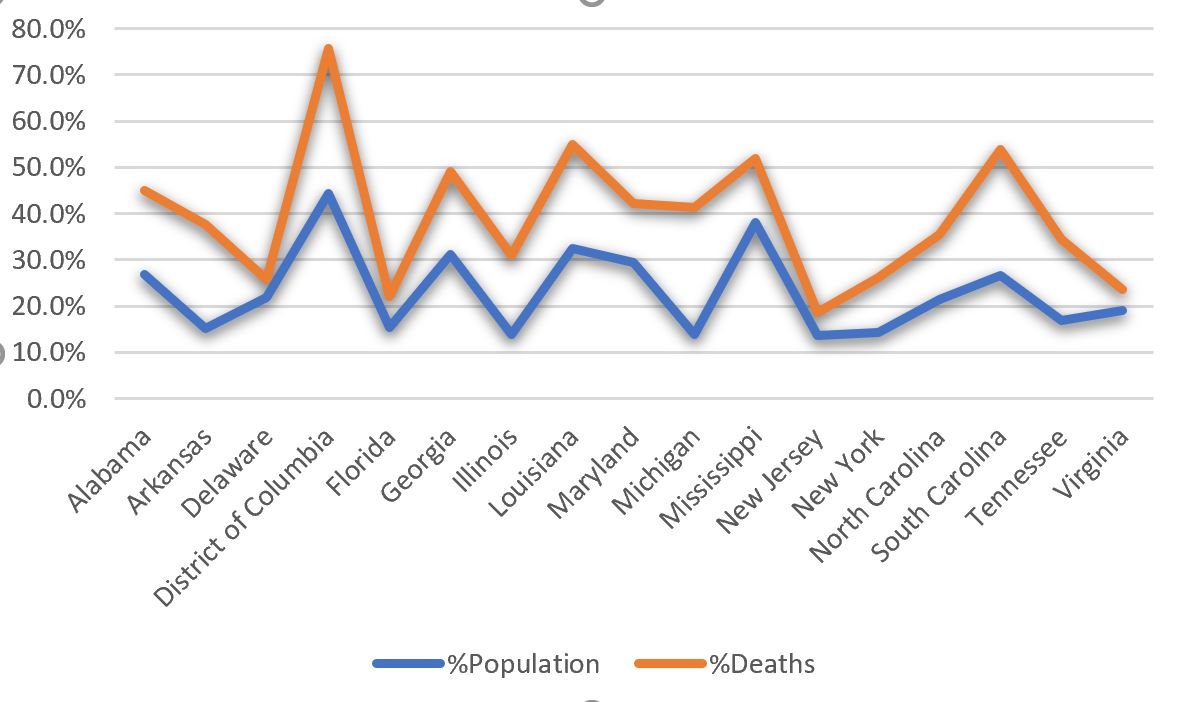
\includegraphics[width=0.4\textwidth]{figures/Deaths vs Pop.jpg}
  \caption{Difference in Death Rates and Population Rates.}
\end{figure}


%Before we get to the actual introduction, welcome to Overleaf, as well as \LaTeX itself! Although \LaTeX certainly has its quirks, we hope that by contrasting the template you see here with the compiled document on the right side, you can get an intuitive sense of how to work with it. Anyhow, let's begin!

%Another thing before the introduction; here, I'm going attach a citation to this sentence \cite{ReferenceName}. Scroll on down to the bibliography section of the \LaTeX\ code if you'd like to see the other end of the built-in references system. The numbering is all handled in-house -- you just have to assign each reference a key, and Overleaf takes care of the rest!

%On with the actual introduction. Here is where you'd introduce the context surrounding your study. What led you to the question you ended up asking? Why is it relevant? Which fields of science is your question based around?

%You could also potentially discuss why Altmetrics themselves are relevant and were important in answering the question your team conceptualized, especially in comparison to using more traditional metrics such as citations.

%While the structure of the previous parts of the introduction can be relatively variable, you must make sure to provide a brief overview of the study itself, and the methods you used to accomplish it. Obviously, excessive detail is not necessary (that's what the next section is for). Lastly, be sure to make mention of the potential implications of your findings, but once again remember that you'll be going into more detail about that in the discussion.

%Also, please do remember that the STEM Fellowship Journal is an open access journal, which means that the full final papers of previous BDC winners are a simple Google search away!

\section{Materials \& Methods}

Open-source data sets were downloaded from multiple COVID Data tracking websites\cite{apm}. Demographic data about different states was downloaded from the APM Research Lab. \cite{cdc} \cite{pollution}
From the data-sets, R was used to generate a list of states where the pandemic was most rampant. Certain demographic data such as population density was also obtained in this manner. However, more essential data was compiled from the government files. 
All the data was then combined further refined in Excel to create a file containing all necessary medical and demographic details about states with above average black populations. 
The final collated data was then analysed using 2 methods in R. First a heat map was created in order to visualize how the 17 states were relative to each other in terms of some socioeconomic variables such as poverty, education, diabetes prevalence etc. as shown in the Figure 2. 
After this, a multi-variable regression was conducted to determine using R to determine the most important factors.
%This is where you talk about the methods used to carry out the study. Be as concise and to-the-point as possible, and remember - \textbf{do not justify your methods here!} You simply need to state what you did. You can (and probably should) mention the purpose of using a certain computational tool within the context of what you set out to achieve, but mentioning things like 'it's particularly efficient at this and better than all competing computational tools' is unnecessary in the methods section. However, you can definitely talk about all of this in the discussion, and talk about why your methods are, say, the most effective ones for the task.

%Think of this section as a technical manual of sorts, that another team of researchers could read and easily follow in order to replicate what you did to carry out this study.

%Because of the straightforward nature of the methods section, this might be the one your team wants to write first. It's essentially you just documenting what your team has already done, which should be no problem to write, since you will already have an established workflow by this point.

\section{Results}

After extracting all the necessary data, we first organized the racial, socioeconomic and health data using Excel through filtering necessary information. A clustered bar graph (Figure 2) of all available states’ death rates of different races was plotted using Excel. 

\begin{figure}
  \centering
  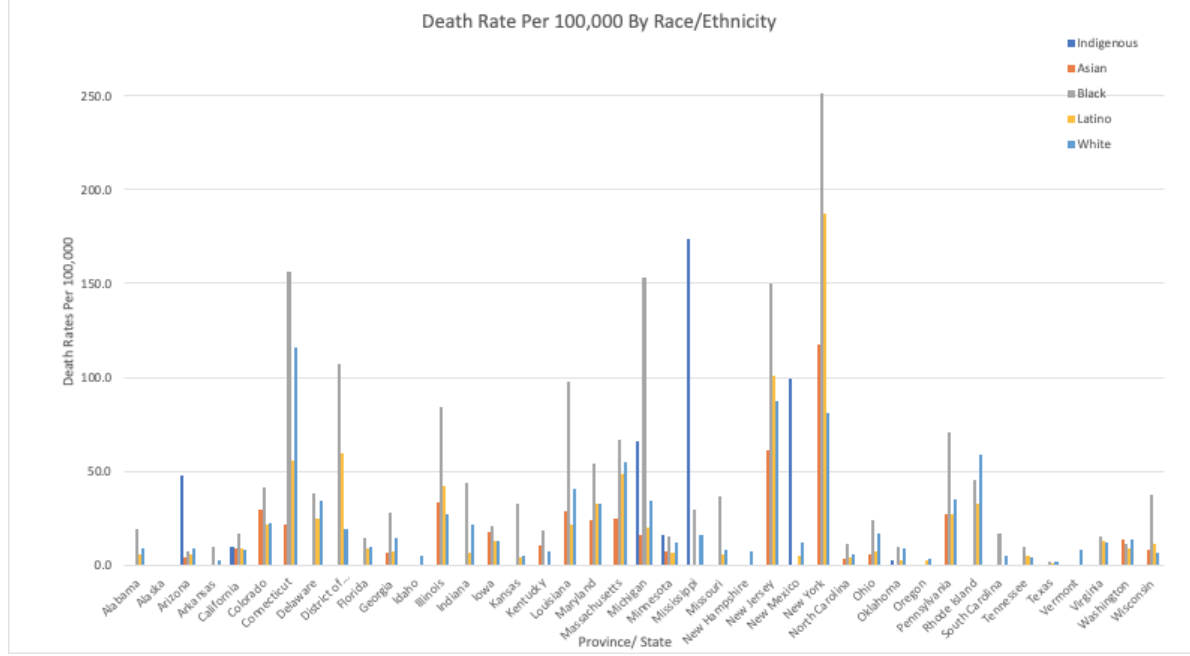
\includegraphics[width=0.4\textwidth]{figures/Flora.png}
  \caption{Death Rates.}
\end{figure} 

It was observed that the black population had the highest death rate per 100,000 for several states. In order for us to better study the effect of socioeconomic and health factors on black population death, we studied all states with greater than average black populations ( > 13\%), which left data for 17 states. 
The final collated data was then analysed using 2 methods in R; first with a heat map, then by creating a multi-variable regression model. This data visualization technique was employed to provide visual cues about the socioeconomic standings of the states as shown in the Figure 3. We observe that District of Columbia ranks towards the higher side of the scale for all variables; unsurprisingly, its black population accounts for almost 49\% of the entire population. Alabama and Arkansas are close with about 27\% and 16\% of the entire population to be black population respectively. 
\begin{figure}
  \centering
  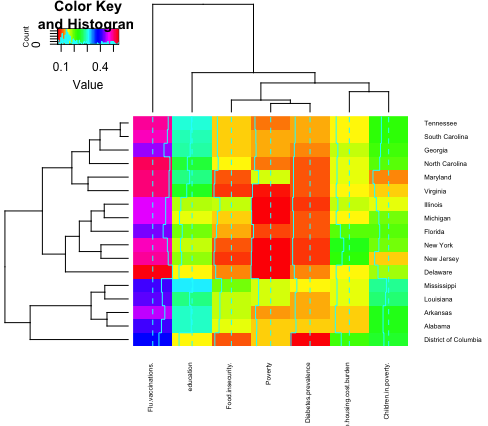
\includegraphics[width=0.4\textwidth]{figures/PLOT.png}
  \caption{State Factors}
\end{figure}
Then, data was analyzed to create a multi-variable regression model, with our y-variable as the Percentage of Black Population Death, and different explanatory x-variables, such as Poverty and Population Density. These variables were added into a multi-variable linear regression model, and variables with p-values greater than an alpha of 0.05 were filtered out as they did not significantly contribute to our model. Additionally, the data was centered by scaling it. Our final regression model is y = 0.39 + 0.08*Black Population\% + 0.09Population Density - 0.10medianhousevalue - 0.10Life Expectancy - 0.08 Diabetes Prevalence, with an adjusted R-squared value of 0.8901. 


%this is the results part
%The results section is probably next easiest to write after the Methods section, since it essentially boils down to presenting your data. If anything, the production of good, high quality figures is the most important and potentially time-consuming part of this. However, make sure to not analyze any of your results here! All of that belongs in the discussion.

%Including figures into \LaTeX\ can seem intimidating at first, but Overleaf makes it easy: simply click the 'Project' button above, select 'Files', and upload away from your computer. Then, insert the file name into the appropriate section of the code below.  Figure 1  shows the output of such code. A pretty good guide to formatting figures can be found at \url{https://en.wikibooks.org/wiki/LaTeX/Floats,_Figures_and_Captions#Figures}.




\section{Discussion}
%We observe that the District of Columbia ranks towards the higher side of the scale for all variables; its black population accounts for almost 49% of the entire population. Alabama and Arkansas are close with about 27% and 16% of the entire population to be black population respectively.  

The multi-variable model suggests that the socioeconomic factors that significantly affect black population death percentage include: Black population \%, Population density, Median House Value, Life Expectancy, and Diabetes Prevalence. Additionally, the intercept of 0.39 proposes that with all socioeconomic variables as 0, the percentage death of black population is 0.39, or 39\% for all states with disproportionate black populations (>13\%).  This is a fairly high percentage and might not be the best interpretation as it assumes that all variables, including life expectancy, are 0 which is not possible. 
Furthermore, our results suggest that both black population and population density are positively correlated to the mortality rate, while Median House Value, life expectancy, and prevalence of diabetes are negatively correlated. Some of these results are rather unusual, especially the results surrounding  Diabetes prevalence, which contradict both our predictions and other trusted research, which shows that they should have a positive correlation.  \cite{diabetes}
Additionally, one major explanatory variable that was predicted would affect the death rate was poverty, but was filtered out of the regression due to it not being statistically significant. This indicates that other socioeconomic and health factors that could have been more pertinent to this study, could have also been excluded. 
It is important to note that our results could have a systematic bias due to the incomplete data provided . Additionally, state based data was utilized for this research as national data was unavailable. The utilisation of  state data leads to a small sample size of 17 states, which likely made the result less resistant to any outliers, and would not represent findings as accurately as country-wide data. Furthermore, findings differ from state to state as each have different rules to what they upload; for example, some states have missing or incomplete racial data, while others combine their race/ethnicity data. Thus, it is difficult to make any complete conclusions.


%nish might wanna refer to this article for some of our arguments : https://www.ncbi.nlm.nih.gov/pmc/articles/PMC4194634/.

%And here is the 'meat' of the paper, so to speak. This is where you interpret your results, pointing out interesting trends within your data and how they relate to your initial hypothesis. This is also the place to justify your methodology, if you're so inclined (i.e. Why did you specifically use a certain statistical test over another? Why this tool over that tool?). Lastly, you're going to want to discuss potential sources of error. Make sure to make explicit reference to figures/tables when discussing your data; it can be helpful to walk the reader through your own personal interpretation of each figure in order. Although we recommend looking at past winning papers over at the STEM Fellowship Journal's website anyways, referring to those papers might prove most helpful when it comes to writing your discussion.

\section*{Conclusions}
%What are the long-term implications of our findings?
%insert paragraph about what we found

It is has been shown that the corona virus has had double the mortality rate for black people than white people \cite{apm}. As of the time of writing, it is hard to ascertain if this is due to mistreatment of black people or simply an unhappy coincidence. If these deaths are the result of systemic racism in America, that is chilling shock to a system which is based on cherished American principles of equal treatment in society. 

This study was conducted to discern if there were non-health related factors that were causing the heightened mortality rates among the black population of USA. Our findings show that the factors such as Life Expectancy and Median House Value are negatively correlated to the mortality rate, but the size of the black population and population density are positively correlated. 

Although the study tried to focus on states with higher than average black populations, further research can be conducted including all the states to see if there are discrepancies among other races as well, such as Asians and Hispanics. It may also be useful to conduct similar studies in countries which has substantial black minorities such as the United Kingdom. This would help ascertain if this pattern is prevalent only in the USA or if it is more widespread. 

%Wrap up your discussion succinctly while pointing out the significance of your work as well as it what it means for the fields you examined as much as possible. Lastly, suggest ideas for future studies that could build on your work, and justify why they might be useful. Otherwise, you're all done!

\section*{Acknowledgements}
First, we would like to thank our mentor, Owen Whitley, for his support and guidance. We would also like to thank the STEM Fellowship for the opportunity to engage in research and access to workshops that would help make our research more meaningful. 

%Anyone to thank/credit for helping your team along the way? This is the place to do it!

\bibliography{bibliography.bib}


\end{document}
